\documentclass[10pt,handout]{beamer}

\usepackage{spot}
\usepackage{color}

\usetheme{Pittsburgh}
\usecolortheme{seahorse}
\useoutertheme{split}

\setbeamertemplate{footline}[split, frame number]
\setbeamertemplate{enumerate items}[default]
\setbeamertemplate{itemize items}[circle]

\newtheorem{comments}{Comments}
\newtheorem{question}{Question}
\newtheorem{goal}{Goal}
\newtheorem{remark}{Remark}
\newtheorem{proposition}{Proposition}
\newtheorem{conjecture}{Conjecture}

\newcommand*\oldmacro{}
\let\oldmacro\insertshorttitle
\renewcommand*\insertshorttitle{
\oldmacro\hfill
\insertframenumber\,/\,\inserttotalframenumber}

%% ----------------------------------------------------------------------  

\begin{document}

\setspotlightstyle{rectangle, rounded corners,fill=structure.fg!25!white,path fading=none}

\title[Inquiry-Based Education in Mathematics]
{\large \textbf{Inquiry-Based Education in Mathematics: Models, Methods, \& Effectiveness for Higher Education}}
\author[D.C.~Ernst and TJ Hitchman]{Dana C.~Ernst, Northern Arizona University\\
Theron J.~Hitchman, University of Northern Iowa}
\institute{\url{http://danaernst.com}\\
\url{http://www.uni.edu/theron/}}

\vspace{1em}

\date{\textbf{Workshop on Innovations in Higher\\ Education Mathematics Teaching}\\
Cardiff University, 7--9 July 2014}

\frame{\titlepage}

\begin{frame}

\vfill
\begin{center}
\spot[inner sep=3.5ex]{{\Huge \textbf{Introductory Questions}}}
\end{center}
\vfill

\end{frame}

%% ----------------------------------------------------------------------

\begin{frame}{\textbf{Question One}}

\begin{center}{\Huge Why are we here?}\end{center}

\end{frame}

\begin{frame}{\textbf{Question One: Sharper Version}}

\begin{center}{\Huge From a learner's perspective, what is the purpose of continuing to study past secondary school?}\end{center}

\end{frame}

\begin{frame}{\textbf{Question Two}}

\begin{center}{\Huge What are the goals of a university education?}\end{center}

\end{frame}

\begin{frame}{\textbf{Question Three}}

\begin{center}{\Huge Information is very free and open these days. Given that one can read and study on one's own, what is the point of going to university?}\end{center}

\end{frame}


\begin{frame}{\textbf{Question Four}}

\begin{center}{\Huge What do you reasonably expect that your students will remember from your courses 20 years later?}\end{center}

\end{frame}

\begin{frame}{\textbf{Question Five}}

\begin{center}{\Huge How does a person learn something new?}\end{center}

\end{frame}

\begin{frame}{\textbf{Question Six}}

\begin{center}{\Huge How should a course of study be structured to facilitate learning?}\end{center}

\end{frame}

\begin{frame}{\textbf{Question Seven}}

{\Large
What are the potential pitfalls? What challenges do we face in building a community where we all engage in collaborative inquiry?}\\[.5in]

Specifically:
\begin{center}{\Huge What barriers would a newcomer encounter that might make them leave such a group?}\end{center}

\end{frame}

\begin{frame}{\textbf{Question Eight}}

\begin{center}{\Huge How do we create a safe space, so that we can all engage in the process with minimum psychological damage?}\end{center}

\end{frame}

%% ----------------------------------------------------------------------

%% WHAT IBL? %%

%% ----------------------------------------------------------------------
\begin{frame}

\vfill
\begin{center}
\spot[inner sep=3.5ex]{{\Huge \textbf{What is IBL?}}}
\end{center}
\vfill

\end{frame}

%% ----------------------------------------------------------------------

\begin{frame}

\begin{block}{The Big Picture}

\vspace{1em}

\spot[inner sep=1ex]{{
\begin{quote}
\textbf{If we really want students to be independent, inquisitive, \& persistent, then we need to provide them with the means to acquire these skills.}
\end{quote}
}}
\end{block}

\end{frame}

%% ----------------------------------------------------------------------

\begin{frame}

\begin{block}{What is inquiry-based learning (IBL)?}
\begin{itemize}
\item<2-> According to the \alert{Academy of Inquiry-Based Learning}:
\begin{itemize}\normalsize
\item<2-> IBL is a teaching method that engages students in sense-making activities.
\item Students are given tasks requiring them to solve problems, conjecture, experiment, explore, create, \& communicate.
\item<2-> Rather than showing facts and/or algorithms, the instructor guides students via well-crafted problems. \pause
\end{itemize}
\item<3-> Often involves very little lecturing, and typically involves student presentations.\pause
\item<4-> Example: Modified Moore Method, after R.L.~Moore. \pause
\item<5-> Students should as much as possible be responsible for:
\begin{itemize}\normalsize
\item<6-> guiding the acquisition of knowledge and,
\item<6-> validating the ideas presented. (Students should not be looking to the instructor as the sole authority.)
\end{itemize}
\end{itemize}
\end{block}

\end{frame}

%% ----------------------------------------------------------------------

\begin{frame}

\begin{block}{Guiding Principle of IBL}
Continually ask yourself the following question:

\vspace{1em}

\spot[inner sep=1ex]{ 
\begin{quote}
\textbf{Where do I draw the line between content I must impart to my students versus content they can produce independently?}
\end{quote}}

\end{block}

\begin{block}<2->{Our Main Objective}
How do we get here?

\begin{center}
\tikzstyle{block} = [rectangle, fill=structure.fg!25!white, text width=6em, text centered, rounded corners, minimum height=2.5em,inner sep=1ex]
\tikzstyle{line} = [draw, very thick, -stealth]
\begin{tikzpicture}
\node [block] (answer) at (0,0) {\textbf{Students answering questions}};
\node [block] (ask) at (4,0) {\textbf{Students asking questions}};
\path [line] (answer) -- (ask);
\end{tikzpicture}
\end{center}
\end{block}

\end{frame}

%% ----------------------------------------------------------------------

\begin{frame}

\begin{block}{Two Typical Approaches/Modes to IBL}
\begin{enumerate}
\item Student presentations.
\item Small group work.
\end{enumerate}
Most IBL instructors implement some combination.
\end{block}

\begin{block}<2->{Important Role Changes}
\begin{itemize}
\item Instructor becomes a mentor, cheerleader, and coach. Focus on teaching process.
\item Student becomes the mathematician.
\end{itemize}
\end{block}

\end{frame}

%% ----------------------------------------------------------------------

\begin{frame}

\begin{block}{IBL vs Presentations/Group Work}
\begin{itemize}
\item Student presentations \& group work act as vehicles for IBL. 
\item Yet student presentations \& group do not imply IBL. 
\item What matters is what is happening during these activities.
\end{itemize}
\end{block}

\begin{block}<2->{IBL vs Inverted/Flipped Pedagogy}
\begin{itemize}
\item<2-> IBL/Moore Method is an instructional practice.
\item<2-> The flipped classroom is:
    \begin{itemize}\normalsize
    \item<2-> A platform, not an instructional practice. 
    \item<2-> Centered around the idea of removing some/all of the information transfer tasks outside of class \& replacing the time that's freed up with whatever instructor feels is appropriate.
    \end{itemize}
\item<2-> IBL and \emph{flipped learning} (see R.~Talbert's talk) are compatible.
\end{itemize}
\end{block}

\end{frame}

%% ----------------------------------------------------------------------

\begin{frame}

\begin{block}{Are you doing IBL?}
\begin{itemize}
\item<2-> Who develops the mathematics which is discussed?
\item<3-> Who presents the mathematics?
\item<4-> Who critiques the mathematics once presented?
\item<5-> Who decides what is correct mathematics?
\item<6-> Who asks the questions that drive further work?
\end{itemize}
\end{block}

\end{frame}

%% ----------------------------------------------------------------------

%% WHY IBL? %%

%% ----------------------------------------------------------------------

\begin{frame}

\vfill
\begin{center}
\spot[inner sep=3.5ex]{{\Huge \textbf{Why IBL?}}}
\end{center}
\vfill

\end{frame}

%% ----------------------------------------------------------------------

\begin{frame}

\begin{block}{One minute version of why IBL}
\begin{itemize}
\item<2-> Our system needs an upgrade.
\item<3-> Unintended negative outcomes via traditional methods.
\item<4-> Research suggests IBL outcomes are better.
\end{itemize}
\end{block}

\vspace{1em}

\spot<5->{{\large \begin{quote}<5->
``Things my students claim that I taught them masterfully, they don’t know." -- Dylan Retsek
\end{quote}}}

\end{frame}

%% ----------------------------------------------------------------------

\begin{frame}

\begin{block}{My IBL origins}
\begin{itemize}
\item<2-> When I started teaching, I mimicked the experiences I had as a student (i.e., I lectured).
\item<3-> By most metrics, I was a successful teacher (e.g., high evaluations, several awards). Why change?
\item<4-> Inspired by a Project NExT Workshop run by Carol Schumacher (Kenyon College), I decided to give IBL a try.
\item<5-> For 3 consecutive semesters, I taught an intro to proof course at Plymouth State University.
\item<6-> 1st two iterations taught via lecture-based approach.
\item<7-> 3rd time taught using IBL with emphasis on collaboration.
\item<8-> When I taught an abstract algebra course containing students from both styles, anecdotal evidence suggested students taught via IBL were stronger proof-writers \& more independent as learners.
\item<9-> I was sold from that moment on.
\end{itemize}
\end{block}

\end{frame}

%% ----------------------------------------------------------------------

\begin{frame}

\begin{columns}[c]
\column{.7\textwidth}
\begin{block}{Some Data}
\begin{itemize}
\item<2-> 2010: 3.7 million students in secondary school. % http://goo.gl/hRixYj
\item<3-> 2010: 52\% of those go to University. % http://goo.gl/hwZHYU
\item<4-> 2013: 38\% of the UK population had a degree. % http://www.ons.gov.uk/ons/dcp171776_337841.pdf
%\item 2013: 47\% of graduates don't take up graduate jobs. % http://goo.gl/eEQRlh
\item<5-> 2010: 16,000 people started a PhD. % http://goo.gl/fcuaqf
\end{itemize}
\end{block}
\column{.2\textwidth}
\begin{center}
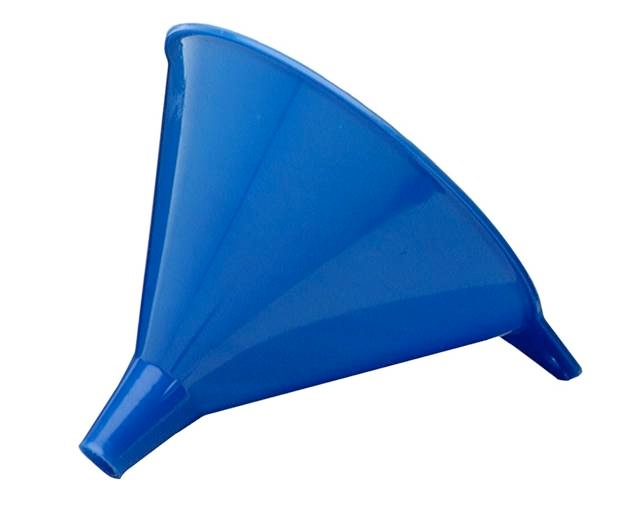
\includegraphics[width=1in]{Funnel.jpg}<6->
\end{center}
\end{columns}

\begin{block}{Conclusion?}<7->
Education is a self-populating institution!
\vspace{1em}
\begin{center}
\spot<8->[inner sep=1.5ex]{{\onslide<8->{\large \textbf{You are peculiar!}}}}
\end{center}
\vspace{1em}
\onslide<8->{We need to renormalize.}

\end{block}

\end{frame}

%% ----------------------------------------------------------------------

\begin{frame}

\begin{block}{What is happening in STEM education?}
\begin{itemize}
\item There exists a growing body of evidence suggesting students are dissatisfied with learning experiences in STEM.
\item Math Education Research suggests that college students have difficulty with:
    \begin{itemize}\normalsize
    \item Solving non-routine problems,
    \item Packing/Unpacking mathematical statements,
    \item Proof.
    \end{itemize}
\end{itemize}

\vspace{1em}

Schoenfeld 1988, Muis 2004, Selden and Selden 1995/1999/2003, Dreyfus 2001, Sowder and Harel 2003, Weber 2001/2003, Weber and Alcock 2004, Tall 1994

\end{block}

\end{frame}

%% ----------------------------------------------------------------------

\begin{frame}

\begin{columns}[c]
\column{.6\textwidth}
\begin{block}{Talking About Leaving}
\begin{itemize}
\item About half of STEM majors switch to non-STEM.
\item Top 4 reasons for switching are teaching related.
\item Good ones leave, too.
\item Loss of interest.
\item Curriculum overload.
\item Students dissatisfied with teaching of STEM classes and less so with non-STEM.
\item Weed-out culture.
\end{itemize}
\end{block}
\column{.3\textwidth}
\begin{center}
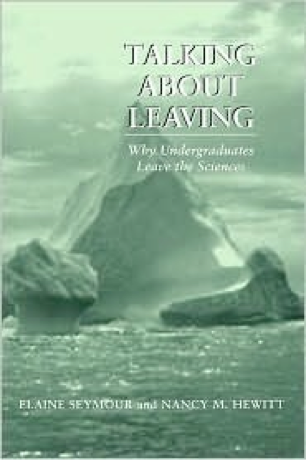
\includegraphics[width=1.25in]{TalkingAboutLeaving.png}
\end{center}
\end{columns}

\vspace{1em}

E.~Seymour, N.M.~Hewitt. \emph{Talking about leaving: Why undergraduates leave the sciences}. Westview Press, 1997.

\end{frame}

%% ----------------------------------------------------------------------

\begin{frame}

\begin{block}{The Good News}
Evidence from the math ed literature suggests that active, learner-centered instruction leads to improved conceptual understanding, problem solving, proof writing, retention, habits of mind, and attitudes about math.

\vspace{1em}

Boaler 1998, Kwon et al. 2005, Rassmussen et al. 2006, Smith 2006, Chappell 2006, Larsen et al. 2011/2013/2014, etc.

\end{block}

\end{frame}

%% ----------------------------------------------------------------------

\begin{frame}

\begin{block}{The Colorado Study by Sandra Laursen et al.}
\begin{itemize}
\item<2-> Quasi-experimental study: Data include 300 hours of classroom observation, 1100 surveys, 110 interviews, 220 tests, and 3200 academic transcripts, gathered from $>100$ course sections at 4 campuses over 2 years.
\item<3-> Statistically significant advantages for students in IBL vs traditional courses.
\end{itemize}
\end{block}

\vspace{-1em}

\onslide<4->{\begin{center}
\tikzstyle{block} = [rectangle, fill=structure.fg!25!white, text width=4em, text centered, rounded corners, minimum height=2.5em]
\tikzstyle{line} = [draw, very thick, stealth-]
\begin{tikzpicture}[scale=.9]
\node [block] (IBL) at (0,2.25) {{\scriptsize \textbf{IBL}}};
\node [block] (interview) at (-5,0) {{\scriptsize \textbf{Interviews}}};
\node [block] (salg) at (-3,0) {{\scriptsize \textbf{SALG}}};
\node [block] (prepost) at (-1,0) {{\scriptsize \textbf{Pre/Post Tests}}};
\node [block] (transcripts) at (1,0) {{\scriptsize \textbf{Transcripts}}};
\node [block] (gender) at (3,0) {{\scriptsize \textbf{Gender}}};
\node [block] (observations) at (5,0) {{\scriptsize \textbf{Observations}}};
\node [block] (non-IBL) at (0,-2.25) {{\scriptsize \textbf{Non-IBL}}};
\path [line] (IBL) -- (salg);
\path [line] (IBL) -- (interview);
\path [line] (IBL) -- (prepost);
\path [line] (IBL) -- (transcripts);
\path [line] (IBL) -- (gender);
\path [line] (IBL) -- (observations);
\end{tikzpicture}
\end{center}}

\end{frame}

%% ----------------------------------------------------------------------

\begin{frame}

\begin{block}{The Twin Pillars}
\begin{enumerate}
\item Deep engagement in rich mathematics,
\item Opportunities to collaborate.
\end{enumerate}
\end{block}

\begin{block}{Laursen et al. 2013}<2->
\emph{``Our study indicates that the benefits of active learning experiences may be lasting and significant for some student groups, with no harm done to others. Importantly, ‘covering’ less material in inquiry-based sections had no negative effect on students' later performance in the major."}
\end{block}

\begin{block}{Laursen et al. 2014}<3->
\emph{``Despite variation in how IBL was implemented, student outcomes are improved in IBL courses relative to traditionally taught courses, as assessed by general measures that apply across course types. Particularly striking, the use of IBL eliminates a sizable gender gap that disfavors women students in lecture-based courses."}
\end{block}

\end{frame}

%% ----------------------------------------------------------------------

\end{document}